\section{Methods \label{chapter2}}
\subsection{KLNMF}
\citet{lee2001algorithms} suggests that \textsc{klnmf} is a \textsc{nmf} that minimising the Kullback-Leibler divergence
\begin{equation*}
  D(V||WH)=\sum_{ij}\left(V_{ij}\log\frac{V_{ij}}{\left(WH\right)_{ij}}-V_{ij}+\left(WH\right)_{ij}\right).
\end{equation*}
Define $C(V_{ij})$ to be arbitrary function of the observed matrix only. As this original matrix V is observed, minimising this Kullback-Leibler divergence is equivalent to minimising
\begin{equation*}
  \sum_{ij}\left(-V_{ij}\log\left(WH\right)_{ij}+\left(WH\right)_{ij}+C(V_{ij})\right).
\end{equation*}
Taking exponential of the negative of this score function, the problem transforms to maximising the following likelihood function
\begin{equation*}
L(WH|V)=\prod_{ij}\left(\left(WH\right)_{ij}^{V_{ij}}e^{-\left(WH\right)_{ij}}+C(V_{ij})\right).
\end{equation*}
Choosing constant $C(V_{ij})$ to be $-\log V_{ij}!$ gives
\begin{equation*}
L(WH|V)=\prod_{ij}\left(\frac{\left(WH\right)_{ij}^{V_{ij}}e^{-\left(WH\right)_{ij}}}{V_{ij}!}\right).
\end{equation*}
Hence, the probability density function of each element of the original matrix~V is Poisson
\begin{equation*}
P(V_{ij})=\frac{\left(WH\right)_{ij}^{V_{ij}}e^{-\left(WH\right)_{ij}}}{V_{ij}!}
\end{equation*}
is a sufficient condition to yield this likelihood. Hence \textsc{klnmf} is most suitable for images with Poisson noise.
\subsection{Asymptotic equivalence of noise distributions}
 We design an Gaussian noise and a Poisson noise with similar magnitude. Poisson distribution with parameter~$\lambda$ (integer) is equivalent to the sum of $\lambda$ Poisson distributions with parameter~$1$ (reference a book!!!!!!!!!!here). Hence for $\lambda$ large, Central Limit Theorem implies that Poisson distribution with parameter~$\lambda$ is well approximated by $N(\lambda,\lambda)$. When applying Poisson noise to an image, we do not degree of freedom to choose any parameter. The variance is the magnitude of the pixels. To fairly compare the robustness of \textsc{klnmf} with \textsc{nmf}, we choose the variance of Gaussian noise to be the magnitude of the pixel, that is, $N(0,V)\approx \operatorname{Poi}(V)-V$. Figure~\ref{noise} visualises the this derivation with $V=40$.
\begin{figure}
  \centering
  % Requires \usepackage{graphicx}
  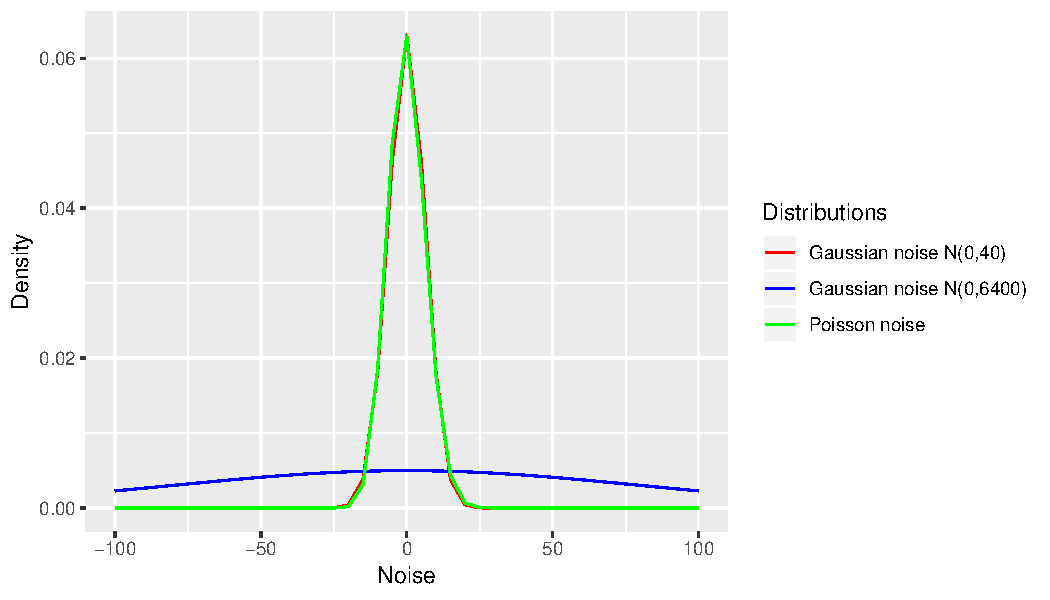
\includegraphics{resource/noise}\\
  \caption{Compare a Gaussian noise~$N(0,40)$ with Poisson noise $\operatorname{Poi}(40)-40$. They two distributions are asymptotically equivalent and have similar density functions.}\label{noise}
\end{figure}

